\providecommand{\main}{../../..}
\documentclass[\main/dresen_thesis.tex]{subfiles}
\renewcommand{\thisPath}{\main/chapters/theoreticalBackground/scattering}
\begin{document}
\section{Scattering}\label{sec:theoreticalBackground:scattering}
Scattering describes the general physical process, where radiation changes its straight path due to interaction with another object.
In a broad perspective this includes all various types of radiation - light, x-ray, electron, neutron, \etc .
For example it includes the very daily process of seeing, where after a light wave is emitted from a source like the sun or a light bulb, the wave is scattered from an object in the room before it is finally detected within ones eye. 
And scattering also includes the process where after a neutron is generated in a nuclear reactor, it interacts with a sample in a experimental hall before it is measured with a sophisticated detector.

In this work, multiple x-ray and neutron scattering techniques are applied to study the nuclear and magnetic structure of nanoparticles and their manufactured assemblies. 
To understand the rich information that is obtained by those techniques, \refsec{sec:theoreticalBackground:scattering:scatteringTheory} presents in the following a brief introduction to the general scattering theory and \refsec{sec:theoreticalBackground:scattering:interactionWithMatter} to the interaction of x-ray and neutrons with matter.
Then the theory behind the mainly applied techniques are discussed: small-angle scattering (\refsec{sec:theoreticalBackground:scattering:SASNanoparticles}), grazing-incidence small-angle scattering (\refsec{sec:theoreticalBackground:scattering:GISAS}) and reflectometry (\refsec{sec:theoreticalBackground:scattering:reflectometry}).
\subsection{Scattering Theory}\label{sec:theoreticalBackground:scattering:scatteringTheory}
Scattering theory describes the scattering of waves and particles from a scattering center as depicted in \reffig{fig:theoreticalBackground:scattering:scatteringTheory:scatteringProcess}. 
\begin{figure}[tb]
  \centering
  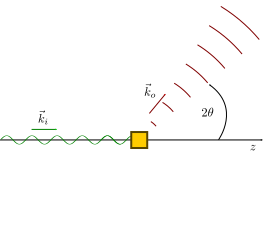
\includegraphics{scatteringTheory_scatterProcess}
  \caption{\label{fig:theoreticalBackground:scattering:scatteringTheory:scatteringProcess}General scattering process. An incoming wave with wave vector $\vec{k}_i$ (green) interacts with a scattering center (yellow) and produces an outgoing wave with wave vector $\vec{k}_o$ (red).}
\end{figure}

An incoming wave $\vec{k}_i$ with defined direction can interact with a scattering center and due to this deviate from its straight path, exiting as outgoing wave $\vec{k}_o$. 
If energy is conserved ($|\vec{k}_i| = |\vec{k}_f|$) the process is called elastic and otherwise inelastic.
The vector describing the change from one vector to the other is conventionally noted by
\begin{align}
  \vec{q} \eq \vec{k}_o - \vec{k}_i.
\end{align}
For an elastic process the magnitude of $\vec{q}$ is directly determined by the wavelength $\lambda$ and angle $2\theta$ between $\vec{k}_i$ and $\vec{k}_o$ by
\begin{align}
  |\vec{q}| \eq \frac{4 \pi}{\lambda} \sin(\theta),
\end{align}
where it is used that $|\vec{k}_i| = \frac{2 \pi}{\lambda}$.

The scattering theory describes the transition probability in dependence of the properties of the incoming wave, scattering center and their interaction potential. 
Thereby it provides the expected scattering intensity for a given model, which can be compared to experimental observations. 
Mathematically, the problem that needs to be solved is the Schr\"odinger equation
\begin{align}
  \label{eq:theoreticalBackground:scattering:scatteringTheory:schrodingerEquation}
  \bigg(\frac{p^2}{2m} + V \bigg) \ket{\psi} \eq E \ket{\psi},
\end{align}
with the boundary condition $V(\vec{r}) \eq 0$ for $\vec{r}$ outside the scattering region. Here it is assumed that the scattering particles are non-interacting, which is a well approximation for photons and neutrons. 
The interaction between the wave and the scattering center is described completely by $V(\vec{r})$ and is discussed in further detail in \refsec{sec:theoreticalBackground:scattering:interactionWithMatter}. 
To solve \refeq{eq:theoreticalBackground:scattering:scatteringTheory:schrodingerEquation}, one defines the Hamiltonians
\begin{align}
  H_0 &\eq \frac{p^2}{2m},\\
  H &\eq H_0 + V,
\end{align}
and define $\ket{\phi}$ as the solution of the free Schr\"odinger equation
\begin{align}
  H_0 \ket{\phi} &\eq E \ket{\phi}.\\
\end{align}
Now, naively, the Schr\"odinger equation can be rearranged as
\begin{align}
  \ket{\psi} &\eq \frac{1}{E - H_0} V \ket{\psi},
\end{align}
but this would not fulfil the boundary condition for $V(\vec{r}) = 0$ and has an ill-defined denominator. 
Therefore, the correct solution needs the addition of the free particle solution and a definition how the pole is supposed to be treated. 
The latter is done by adding a infinitely small and positively complex value $i\epsilon$ to the denominator. The resulting equation
\begin{align}
  \ket{\psi} &\eq \ket{\phi} +  \frac{1}{E - H_0 + i \epsilon} V \ket{\psi},
\end{align}
is known as the Lippmann-Schwinger equation and it solves the Schr\"odinger equation by construction. 
In position space, it reads as integral equation
\begin{align}
  \psi (\vec{r}) &\eq \phi(\vec{r}) + \int \dint \vec{r}^\prime \bra{\vec{r}}\frac{1}{E - H_0 + i \epsilon} \ket{\vec{r}^\prime} V (\vec{r}^\prime)\psi (\vec{r}^\prime),
\end{align}
where it is used that the single-particle potential is diagonal in position space $\bra{\vec{r}} V \ket{\vec{r}^\prime} = V(\vec{r}) \delta(\vec{r} - \vec{r}^\prime)$. 
The solution for the free Hamiltonian is given by as a plane wave solution
\begin{align}
  \phi(\vec{r}) \eq e^{i\vec{k} \cdot \vec{r}},
\end{align}
and the matrix element within the integral is solved by
\begin{align}
  \bra{\vec{r}}\frac{1}{E - H_0 + i \epsilon} \ket{\vec{r}^\prime} \eq -\frac{2m}{4 \pi \hbar^2} \frac{e^{ik|\vec{r} - \vec{r}^\prime|}}{|\vec{r} - \vec{r}^\prime|}.
\end{align}
Thus the integral representation of the Lippmann-Schwinger equation is
\begin{align}
  \psi (\vec{r}) &\eq e^{i\vec{k} \cdot \vec{r}} - \frac{2m}{4 \pi\hbar^2} \int \dint \vec{r}^\prime \frac{e^{ik|\vec{r} - \vec{r}^\prime|}}{|\vec{r} - \vec{r}^\prime|} V (\vec{r}^\prime)\psi (\vec{r}^\prime).
\end{align}
The resulting wave function can be nicely interpret as a superposition of the incoming plane wave with spherical waves generated at $\vec{r}^\prime$, modulated by the interaction potential $V(\vec{r}^\prime)$ and the wave field at this point.
In a standard experimental setup, the detector is often at a position that is far away relative to the scattering volume $r^\prime \ll r$. 
Therefore a good approximation and large simplification in calculation is
\begin{align}
  |\vec{r} - \vec{r}^\prime| \eq r - \frac{\vec{r} \cdot \vec{r}^\prime}{r} + \mathcal{O}\bigg(\frac{{r^\prime}^2}{r}\bigg),\\
  \frac{1}{|\vec{r} - \vec{r}^\prime|} \eq \frac{1}{r} + \mathcal{O}\bigg(\frac{r^\prime}{r^2} \bigg),
\end{align}
then the Lippmann-Schwinger equation reads
\begin{align}
  \psi (\vec{r}) &\eq e^{i\vec{k} \cdot \vec{r}} - \frac{2m}{4 \pi\hbar^2} \frac{e^{ikr}}{r} \int \dint \vec{r}^\prime e^{-i\vec{k}^\prime \cdot \vec{r}^\prime} V (\vec{r}^\prime)\psi (\vec{r}^\prime),
\end{align}
where it was again used that the detector is far away relative to the sample size and thus the outgoing wave points essentially into the direction of the detector  $\vec{k}^\prime = k \vec{r} / r$.

The Lippmann-Schwinger equation can be used to solve the scattering problem for any potential $V$ iteratively by starting on the right hand side of the equation with the free particle solution for $\psi (\vec{r})$ and then putting the solution back into the Lippmann-Schwinger equation, \etc.
The first iteration 
\begin{align}
  \psi (\vec{r}) &\eq e^{i\vec{k} \cdot \vec{r}} - \frac{2m}{4 \pi\hbar^2} \frac{e^{ikr}}{r} \int \dint \vec{r}^\prime e^{-i\vec{q} \cdot \vec{r}^\prime} V (\vec{r}^\prime),\label{eq:theoreticalBackground:scattering:scatteringTheory:firstBornApproximation}
\end{align}
is known as the Born approximation and is the starting point for many further calculations. It fully describes the case where the wave undergoes only a single scattering event as it passes through the sample. 

\subsection{Interaction of X-rays and Neutrons with Matter}\label{sec:theoreticalBackground:scattering:interactionWithMatter}
To solve the Lippmann-Schwinger equation it is necessary to know how the scattering wave and the sample interact with each other, which is represented by the potential $V$. In the case of x-rays, the dominant coupling to consider is the interaction of the x-ray photons with the electron shells of the atoms making up the material. For neutrons however the coupling to the electrons is negligible in contrast to the interaction with the nucleus of the atoms. In the following both interactions and how to evaluate them for different materials is presented in more detail.

...
\subsection{Small-Angle Scattering from Nanoparticles}\label{sec:theoreticalBackground:scattering:SASNanoparticles}
Small-angle scattering is a technique to study nanometer sized objects when the wavelength of the scattered particle is in the order of a few {\aa}ngstr\"om. 
Here, the forward scattering of a collimated beam through a sample is measured on a position sensitive detector around an opening angle in the order of $2 \theta \eq 0.1^\circ - 10^\circ$. 
As the magnitude of the scattering vector $q$ is proportional to $\sin(\theta)$ and $q$ is inversely proportional to the probed length scale, smaller scattering angles $\theta$ mean that larger length scales are probed. 

In the following, the application of small-angle scattering to the study of nanoparticles in dispersion is described. 
In a first step, let's consider for that the sample consists of monodisperse nanoparticles in dispersion. 
The potential $V(\vec{r})$ in the Born approximation formula \refeq{eq:theoreticalBackground:scattering:scatteringTheory:firstBornApproximation} can be written as the sum of a constant background $V_m$ for the solvent and a position dependant potential for the nanoparticles $V_{np}$ in the solvent. The nanoparticle potential can be further rewritten as convolution of a potential $V_{p}(\vec{r})$ describing a single nanoparticle in the solvent and a function $s(\vec{r})$ describing the position of the nanoparticles. In total, we get
\begin{align}
  V(\vec{r}) \eq V_{m} + (s * V_{p})(\vec{r}),\\
  s(\vec{r}) \eq \sum_i \delta(\vec{r} - \vec{r}_i).
\end{align}
Inserting this into the integral, the integral over the constant term is essentially a definition of $\delta (\vec{q})$ and can be ignored as it is 0 for $\vec{q} \neq 0$ and the convolution theorem helps to turn the integral over a convolution to a product of integrals
\begin{align}
  \int \dint \vec{r} e^{-i\vec{q} \cdot \vec{r}} (s * V_{p})(\vec{r}) = \bigg[\int \dint \vec{r} e^{-i\vec{q} \cdot \vec{r}} s(\vec{r})\bigg] \bigg[\int \dint \vec{r} e^{-i\vec{q} \cdot \vec{r}} V_{p}(\vec{r}) \bigg].
\end{align}
The first factor is called the structure factor and the second the form factor. Where the latter describes the scattering due to the shape and properties of the nanoparticle, the first modulates the scattering due to the relative positions. 
\subsection{Grazing Incidence Small-Angle Scattering from a Surface}\label{sec:theoreticalBackground:scattering:GISAS}
\subsection{Reflectometry}\label{sec:theoreticalBackground:scattering:reflectometry}
\end{document}